\subsection{Poincaré-Birkhoff-Witt 定理}

定理 1. 设 \(\mathfrak{g}\) 是李 K-代数，\(U\) 是其包络代数，G 是滤过代数 U 的关联分次代数，S 是 K-模 \(\mathfrak{g}\) 的对称代数。若 \(\mathfrak{g}\) 是自由 K-模，则典范同态 \(\omega: \mathrm{S} \to \mathrm{G}\) 是同构。

令 \((x_{\lambda})_{\lambda \in \Lambda}\) 为 K-模 g 的一个基；给 \(\Lambda\) 赋予全序（Set Theory, Chapter III, § 2, no. 3, Theorem 1）。令 P 为多项式代数 \(\mathrm{K}[z_{\lambda}]_{\lambda \in \Lambda}\)，其不定元 \(z_{\lambda}\) 与 \(x_{\lambda}\) 一一对应。对于 \(\mathrm{M} = (\lambda_1, \lambda_2, \ldots, \lambda_n)\) 中元素组成的每个序列 \(\Lambda\)，令 \(z_{\mathrm{M}}\) 表示单项式 \(z_{\lambda_1}z_{\lambda_2}\ldots z_{\lambda_n}\)，令 \(x_{\mathrm{M}}\) 表示张量 \(x_{\lambda_1}\otimes x_{\lambda_2}\otimes \dots \otimes x_{\lambda_n}\)。

当  递增时，\(z_{\mathbb{M}}\) 构成 K-模 \(\mathbf{M}\)\(\mathbf{P}\) 的一个基（约定 \(\varnothing\) 是递增序列，且 \(z_{\varnothing} = 1\)）。令 \(\mathbf{P}_p\) 为次数 \(\leqslant p\) 的多项式组成的子模。我们先证明若干引理。（为简便起见，若对序列 M 的每个指标  都有 ，就写作 \(\lambda \leqslant M\)\(\lambda \leqslant \mu\)\(\mu\)。）

引理 1. 对每个整数 \(p \geqslant 0\)，存在唯一的从 K-模 \(f_p\)\(\mathfrak{g} \otimes_{\mathbb{K}} \mathrm{P}_p\) 到 K-模 \(\mathrm{P}\) 的同态 ，满足下列条件：

\[
\left(\mathrm{A} _ {p}\right) \quad f _ {p} \left(x _ {\lambda} \otimes z _ {\mathrm{M}}\right) = z _ {\lambda} z _ {\mathrm{M}} \quad \text {   for   } \lambda \leqslant \mathrm{M}, z _ {\mathrm{M}} \in \mathrm{P} _ {p};
\]

\[
\left(\mathrm{B} _ {p}\right) \quad f _ {p} \left(x _ {\lambda} \otimes z _ {\mathrm{M}}\right) - z _ {\lambda} z _ {\mathrm{M}} \in \mathrm{P} _ {q} \quad for \quad z _ {\mathrm{M}} \in \mathrm{P} _ {q}, q \leqslant p;
\]

\[
\left(\mathrm{C} _ {p}\right) \quad f _ {p} \left(x _ {\lambda} \otimes f _ {p} \left(x _ {\mu} \otimes z _ {\mathrm{N}}\right)\right) = f _ {p} \left(x _ {\mu} \otimes f _ {p} \left(x _ {\lambda} \otimes z _ {\mathrm{N}}\right)\right) + f _ {p} \left(\left[ x _ {\lambda}, x _ {\mu} \right] \otimes z _ {\mathrm{N}}\right)
\]

对 \(z_{\mathbf{N}} \in \mathbf{P}_{p-1}\) 成立。（\((\mathbf{C}_p)\) 中出现的各项由 \((\mathbf{B}_p)\) 可知有意义。）

此外，\(f_{p}\) 在 \(\mathfrak{g} \otimes \mathrm{P}_{p-1}\) 上的限制与 \(f_{p-1}\) 一致。

最后一个断言由其余断言推出，因为 \(f_{p}\) 在 \(\mathfrak{g} \otimes_{\mathbb{K}} \mathrm{P}_{p-1}\) 上的限制满足条件 \((\mathrm{A}_{p-1})\)、\((\mathrm{B}_{p-1})\) 和 \((\mathrm{C}_{p-1})\)。我们对 p 归纳证明 \(f_{p}\) 的存在性和唯一性。当 \(p\)\(p = 0\) 时，条件 \((\mathrm{A}_0)\) 给出 \(f_0(x_\lambda \otimes 1) = z_\lambda\)，此时条件 \((\mathrm{B}_0)\) 和 \((\mathrm{C}_0)\) 显然满足。现在假设 \(f_{p-1}\) 的存在性和唯一性已经证明。我们说明，\(f_{p-1}\) 有唯一延拓 \(f_{p}\) 到 \(\mathfrak{g} \otimes_{\mathbb{K}} \mathrm{P}_{p}\)，并满足条件 \((\mathrm{A}_{p})\)、\((\mathrm{B}_{p})\) 和 \((\mathrm{C}_{p})\)。

对于含 p 个元素的递增序列 M，我们必须定义 \(f_{p}(x_{\lambda} \otimes z_{\mathbb{M}})\)。

若 \(\lambda \leqslant M\)，其值由条件 \((A_p)\) 给出。否则，M 可唯一写成 \(M\)\((\mu, N)\) 的形式，其中 \(\mu < \lambda\)、\(\mu \leqslant N\)。于是

\[
z _ {\mathrm{M}} = z _ {\mu} z _ {\mathrm{N}} = f _ {p - 1} (x _ {\mu} \otimes z _ {\mathrm{N}})
\]

由 \((\mathrm{A}_{p - 1})\)，所以 \((\mathrm{C}_p)\) 的左端就是 \(f_{p}(x_{\lambda}\otimes z_{\mathbb{M}})\)。现在 \((\mathrm{C}_p)\) 的右端已经定义好：根据 \((\mathrm{B}_{p - 1})\)，可写为：

\[
f _ {p} (x _ {\lambda} \otimes z _ {\mathrm{N}}) = f _ {p - 1} (x _ {\lambda} \otimes z _ {\mathrm{N}}) = z _ {\lambda} z _ {\mathrm{N}} + w
\]

其中 \(w \in \mathbf{P}_{p-1}\)；因此 \((\mathbf{C}_p)\) 的右端变为：

\[
z _ {\lambda} z _ {\mu} z _ {N} + f _ {p - 1} (x _ {\mu} \otimes w) + f _ {p - 1} ([ x _ {\lambda}, x _ {\mu} ] \otimes z _ {N}).
\]

这样便唯一确定了 \(f_{p}\)，且显然满足条件 \((\mathbf{A}_{p})\) 和 \((\mathbf{B}_{p})\)。当 \((\mathbf{C}_{p})\)\(\mu < \lambda\)、\(\mu \leqslant N\) 时，条件  成立。由于 \([x_{\mu}, x_{\lambda}] = -[x_{\lambda}, x_{\mu}]\)，当 \((\mathbf{C}_{p})\)\(\lambda < \mu\)、\(\lambda \leqslant N\) 时，条件 \((\mathbf{C}_{p})\) 也成立。当 \(\lambda = \mu\) 时 \((\mathbf{C}_{p})\) 显然成立，所以只要 \(\lambda \leqslant N\) 或 \(\mu \leqslant N\)， 就成立。若这些不等式均不成立，则 \(N = (\nu, Q)\)，其中 \(\nu \leqslant Q\)、\(\nu < \lambda\)、\(\nu < \mu\)。以下简写 \(f_{p}(x \otimes z) = xz\)（其中 \(x \in g\)、\(z \in P_{p}\)），由归纳假设有：

\[
x _ {\mu} z _ {N} = x _ {\mu} (x _ {\nu} z _ {Q}) = x _ {\nu} (x _ {\mu} z _ {Q}) + [ x _ {\mu}, x _ {\nu} ] z _ {Q}.
\]

现在 \(x_{\mu}z_{\mathbf{Q}}\) 具有 \(z_{\mu}z_{\mathbf{Q}} + w\) 的形式，其中 \(w\in \mathrm{P}_{p - 2}\)。由于  且 ，可将 (C \(_{p}\) ) 应用于 \(x_{\lambda}(x_{\nu}(z_{\mu}z_{\mathbf{Q}}))\)；根据归纳假设，也可应用于 \(\nu \leqslant Q\)\(\nu < \mu\)\(x_{\lambda}(x_{\nu}w)\)，因而可应用于 \(x_{\lambda}(x_{\nu}(x_{\mu}z_{\mathbf{Q}}))\)。因此：

\[
\begin{array}{r l} x _ {\lambda} (x _ {\mu} z _ {N}) = x _ {\nu} (x _ {\lambda} (x _ {\mu} z _ {\mathbb {Q}})) & + [ x _ {\lambda}, x _ {\nu} ] (x _ {\mu} z _ {\mathbb {Q}}) + [ x _ {\mu}, x _ {\nu} ] (x _ {\lambda} z _ {\mathbb {Q}}) \\ & + [ x _ {\lambda}, [ x _ {\mu}, x _ {\nu} ] ] z _ {\mathbb {Q}}. \end{array}
\]

交换 \(\lambda\) 与 \(\mu\) 后相减：

\[
\begin{array}{r l} {x _ {\lambda} (x _ {\mu} z _ {N}) - x _ {\mu} (x _ {\lambda} z _ {N})} & {= x _ {\nu} (x _ {\lambda} (x _ {\mu} z _ {Q}) - x _ {\mu} (x _ {\lambda} z _ {Q}))} \\ & {\quad + [ x _ {\lambda}, [ x _ {\mu}, x _ {\nu} ] ] z _ {Q} - [ x _ {\mu}, [ x _ {\lambda}, x _ {\nu} ] ] z _ {Q}} \\ & {= x _ {\nu} ([ x _ {\lambda}, x _ {\mu} ] z _ {Q}) + [ x _ {\lambda}, [ x _ {\mu}, x _ {\nu} ] ] z _ {Q} + [ x _ {\mu}, [ x _ {\nu}, x _ {\lambda} ] ] z _ {Q}} \\ & {= [ x _ {\lambda}, x _ {\mu} ] (x _ {\nu} z _ {Q}) + ([ x _ {\nu}, [ x _ {\lambda}, x _ {\mu} ] ]} \\ & {\quad + [ x _ {\lambda}, [ x _ {\mu}, x _ {\nu} ] ] + [ x _ {\mu}, [ x _ {\nu}, x _ {\lambda} ] ]) z _ {Q}} \end{array}
\]

从而由 Jacobi 恒等式

\[
x _ {\lambda} (x _ {\mu} z _ {N}) - x _ {\mu} (x _ {\lambda} z _ {N}) = [ x _ {\lambda}, x _ {\mu} ] z _ {N}
\]

这就完成了引理 1 的证明。

引理 2. 存在从  到  的 \(\alpha\)-映射 \(\sigma\)\(\mathfrak{g}\)\(\mathcal{L}_{\mathbf{K}}(\mathbf{P})\)，使得：

\begin{enumerate}
\def\labelenumi{(\arabic{enumi})}
\item
  \(\sigma(x_{\lambda})z_{\mathbf{M}} = z_{\lambda}z_{\mathbf{M}}\) 对 \(\lambda \leqslant \mathbf{M}\) 成立；
\item
  \(\sigma(x_{\lambda})z_{\mathbf{M}} \equiv z_{\lambda}z_{\mathbf{M}} (\mathrm{mod.~P}_{p})\) 若 \(\mathbf{M}\) 含有 \(p\) 个元素。
\end{enumerate}

由引理 1，对所有 p，存在从 K-模  到 P 的同态 \(f\)，满足条件 \(\mathfrak{g} \otimes_{\mathbb{K}} \mathrm{P}_p\)\(p\)\((\mathrm{A}_p), (\mathrm{B}_p), (\mathrm{C}_p)\)（以 f 替代 \(f_p\)）。此同态定义了从 K-模 \(f\)\(\sigma\)\(\mathfrak{g}\) 到 K-模 \(\mathcal{L}_{\mathbb{K}}(\mathrm{P})\) 的同态 \(\sigma\)，并且由于条件 \(\alpha\)\((\mathrm{C}_p)\)，\(\sigma\) 是 -映射。最后，由于条件 \((\mathrm{A}_p)\) 和 \((\mathrm{B}_p)\)， 满足本引理的性质 (1) 和 (2)。

引理 3. 设 \(t\) 是 \(\mathrm{T}_n \cap \mathrm{J}\) 中的张量。t 的 n 阶齐次分量 \(t_n\) 属于典范同态 \(t\)\(n\)\(\mathrm{T} \to \mathrm{S}\) 的核 I。

我们将 \(t_n\) 写成 \(\sum_{i=1}^{r} x_{\mathrm{M}_i}\) 的形式，其中 \(\mathrm{M}_i\) 是由 \(n\)\(\Lambda\) 中 n 个元素组成的序列。映射 \(\sigma\) 延拓为从代数 T 到代数 \(T\)\(\mathcal{L}_K(P)\) 的同态（仍记为 \(\sigma\)），并且在 \(J\) 上为零。由引理 2，\(\sigma(t)\) . 1 是一个多项式，其最高次数的项为 \(\sum_{i=1}^{r} z_{\mathrm{M}_i}\)。由于 \(t \in J\)，\(\sigma(t) = 0\)，所以在 P 中 \(\sum_{i=1}^{r} z_{\mathrm{M}_i} = 0\)。现在，由于 g 具有基 \(P\)\(P\)\(S\)\(g\)\((x_\lambda)\)，P 自然地与 S 相同。因此 \(t_n\) 在 S 中的典范像为零，即 \(S\)\(t_n \in I\)。

现在可以证明定理 1。必须证明从 S 到 G 的典范同态是单射。换言之，若 \(t \in \mathrm{T}^n\)，\(\psi\) 表示从 T 到 U 的典范满同态，就必须证明条件 \(\psi(t) \in \mathrm{U}_{n-1}\) 蕴含 \(t \in I\)。现在，\(\psi(t) \in \mathrm{U}_{n-1}\) 意味着存在 \(t' \in \mathrm{T}_{n-1}\) 中的张量，使 \(t - t' \in J\)。张量 \(t - t'\) 以 t 作为 n 阶齐次分量，因此由引理 3 有 \(t\)\(n\)\(t \in I\)。

推论 1. 设 \(\mathfrak{g}\) 是自由 K-模。令 W 为 \(\mathbf{T}^n\) 的子 K-模。

若按图 (3) 的记号，\(\tau_{n}\) 在 W 上的限制是从 W 到 \(\mathbf{S}^n\) 的同构，则 \(\psi_{n}\) 在 W 上的限制是从 W 到  中 \(\mathbf{U}_{n-1}\)\(\mathbf{U}_n\) 的一个补空间的同构。

\(\omega_{n} \circ \tau_{n}\) 在 W 上的限制是从 W 到 \(G^{n}\) 的双射；\(\theta_{n} \circ \psi_{n}\) 在 W 上的限制也如此。故推论得证。

推论 2. 若 \(\mathfrak{g}\) 是自由 K-模，则 \(\mathfrak{g}\) 到其包络代数的典范映射是单射。

取 \(\mathbf{W} = \mathbf{T}^1\) 后由推论 1 得到。

当 g 是自由 K-模时（特别是当 K 为域时），在 g 到 U 的典范映射下，将 g 与 U 的一个子模相同。从下面的推论开始采用这一约定。

推论 3. 若 \(\mathfrak{g}\) 有一个全序基 \((x_{\lambda})_{\lambda \in \Lambda}\)，则包络代数  的元素 \(x_{\lambda_1}x_{\lambda_2}\ldots x_{\lambda_n}\)（其中 \(\mathbf{U}\)\((\lambda_1,\dots ,\lambda_n)\) 是 \(\Lambda\) 中元素组成的任意有限递增序列）构成 K-模 \(\mathbf{U}\) 的一个基。

令 \(\Lambda_{n}\) 为 \(n\)\(\Lambda\) 中 n 个元素的递增序列的集合。对 \(\mathrm{M} = (\lambda_1, \ldots, \lambda_n) \in \Lambda_n\)，令 \(y_{\mathrm{M}} = x_{\lambda_1} \otimes x_{\lambda_2} \otimes \dots \otimes x_{\lambda_n}\)。令 \(\mathrm{W}\) 为以  为基的 \(\mathrm{T}^n\) 的子模。推论 1 表明，\((y_{\mathrm{M}})_{\mathrm{M} \in \Lambda_n}\)\(\psi_n\) 在 \(\mathrm{W}\) 上的限制是从 \(\mathrm{W}\) 到  中 \(\mathrm{U}_{n-1}\)\(\mathrm{U}_n\) 的一个补空间的同构。但

\[
\psi_ {n} (y _ {\mathrm{M}}) = x _ {\lambda_ {1}} x _ {\lambda_ {2}} \dots x _ {\lambda_ {n}},
\]

由此推论得证。

推论 4. 令 \(S'^{n} \subset T^n\)\(n\)\(K\) 为 n 阶齐次对称张量的集合。设 K 是特征为 0 的域。则典范映射的复合映射

\[
\mathrm{S} ^ {n} \rightarrow \mathrm{S} ^ {\prime n} \rightarrow \mathrm{U} _ {n}
\]

是从向量空间 \(\mathbf{S}^n\) 到  中 \(\mathbf{U}_{n-1}\)\(\mathbf{U}_n\) 的一个补空间的同构。

取 \(W = S'^n\) 后由推论 1 得到。

以下设 \(\mathbf{K}\) 是特征为 0 的域。令 \(\eta_{n}\) 为刚才定义的从 \(S^n\) 到 \(U_n\) 的映射。令 \(U^n = \eta_n(S^n)\)。向量空间 U 是各 \(U\)\(U^n\) 的直和。各 \(\eta_{n}\) 定义了从向量空间 \(\eta\)\(S = \sum_{n} S^n\) 到向量空间 \(U = \sum_{n} U^n\) 的同构 \(S\)\(U\)，称为从 S 到 U 的典范同构；这不是代数同构。我们有交换图：

\pandocbounded{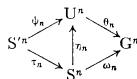
\includegraphics[keepaspectratio]{images/part001_756df219.jpg}}

其中每个箭头表示向量空间同构。若 \(x_{1}, x_{2}, \ldots, x_{n}\) 属于 \(g\)，则 \(\eta_{n}\) 将在 S 中计算的乘积 \(x_{1}x_{2}\ldots x_{n}\) 映到元素

\[
\frac {1}{n !} \sum_ {\sigma \in \mathfrak {S} _ {n}} x _ {\sigma (1)} x _ {\sigma (2)} \dots x _ {\sigma (n)}
\]

该元素在 U 中计算。

推论 5. 设 \(\mathfrak{h}\) 是李代数 \(\mathfrak{g}\) 的子代数，\(\mathrm{U}'\) 是其包络代数。假设 K-模 \(\mathfrak{h}\) 和 \(\mathfrak{g} / \mathfrak{h}\) 是自由的（例如 K 为域时）。令 \(\mathrm{K}\)\((x_{\alpha})_{\alpha \in \mathbb{L}}\) 为 \(\mathfrak{h}\) 的一个基，\((y_{\beta})_{\beta \in \mathbb{M}}\) 为 \(\mathfrak{g}\) 中的一族元素，使它们在 \(\mathfrak{g} / \mathfrak{h}\) 中的典范像构成 \(\mathfrak{g} / \mathfrak{h}\) 的一个基。

\begin{enumerate}
\def\labelenumi{(\alph{enumi})}
\item
  从 \(\mathbf{U}'\) 到 \(\mathbf{U}\) 的典范同态是单射。
\item
  若 \(\mathbf{M}\) 全序，则元素 \(y_{\beta_1} \ldots y_{\beta_q}\)（其中 \(\beta_1 \leqslant \cdots \leqslant \beta_q\)）构成把 \(\mathbf{U}\) 视为 \(\mathbf{U}'\) 的左模或右模时的一个基。
\end{enumerate}

给 \(L \cup M\) 赋予全序，使 L 中每个元素都小于 M 中每个元素。在  中计算的元素 \(x_{\alpha_{1}}x_{\alpha_{2}}\ldots x_{\alpha_{p}}\)（其中 \(U'\)\(\alpha_{1} \leqslant \cdots \leqslant \alpha_{p}\)）构成 \(U'\) 的一个基（推论 3）。元素

\[
x _ {\alpha_ {1}} \dots x _ {\alpha_ {p}} y _ {\beta_ {1}} \dots y _ {\beta_ {q}}
\]

在 U 中计算的这些元素（其中 \(\alpha_{1} \leqslant \cdots \leqslant \alpha_{p} \leqslant \beta_{1} \leqslant \cdots \leqslant \beta_{q}\)）同样构成 U 的一个基。因此，U' 到 U 的典范同态将 U' 的一个基中的元素映到 U 中线性无关的元素，因而是单射。此外可见，\(y_{\beta_1} \ldots y_{\beta_q}\)（其中 \(\beta_{1} \leqslant \cdots \leqslant \beta_{q}\)）构成把 U 视为左 U'-模时的一个基。给  排序，使 M 中每个元素都小于 L 中每个元素，同样可见，\(y_{\beta_1} \ldots y_{\beta_q}\)（其中 \(\beta_{1} \leqslant \cdots \leqslant \beta_{q}\)）构成把 U 视为右 U'-模时的一个基。

在推论 5 的条件下，通过 U' 到 U 的典范同态，将 U' 与 U 中由 h 生成的子代数相同。

推论 6. 假设 K-模 g 是子代数 \(g_{1}, g_{2}, \ldots, g_{n}\) 的直和，且每个 \(g_{i}\) 都是自由 K-模。令 \(U_{i}\) 为 \(g_{i}\) 的包络代数（\(1 \leqslant i \leqslant n\)）。令 \(\phi\) 为从 K-模 \(U_{1} \otimes_{K} \cdots \otimes_{K} U_{n}\) 到 U 的 K-线性映射，它由从  到 U 的多线性映射（\(u_{1}, \ldots, u_{n}\)）\(\mapsto u_{1} \ldots u_{n}\) 定义。则 \(U_{1} \times \cdots \times U_{n}\)\(\phi\) 是 K-模同构。

令 \((x_{\lambda}^{i})_{\lambda \in L_{i}}\) 为 \(g_{i}\) 的一个基。给 \(L_{1} \cup \cdots \cup L_{n}\) 赋予全序，使当  时 \(L_{i}\) 中每个元素都大于 \(L_{j}\)\(i \geqslant j\) 中每个元素。则元素：

\[
\left(x _ {\lambda_ {1}} ^ {1} x _ {\lambda_ {2}} ^ {1} \dots x _ {\lambda_ {p}} ^ {1}\right) \otimes \dots \otimes \left(x _ {\nu _ {1}} ^ {n} x _ {\nu _ {2}} ^ {n} \dots x _ {\nu _ {q}} ^ {n}\right),
\]

其中 \(\lambda_{1}\leqslant\lambda_{2}\leqslant\cdots\leqslant\lambda_{p}\leqslant\cdots\leqslant\nu_{1}\leqslant\nu_{2}\leqslant\cdots\leqslant\nu_{q}\)，构成 \(U_{1}\otimes_{K}\cdots\otimes_{K}U_{n}\) 的一个基。它们经 \(\phi\) 映到元素：

\[
x _ {\lambda_ {1}} ^ {1} x _ {\lambda_ {2}} ^ {1} \dots x _ {\lambda_ {p}} ^ {1} \dots x _ {\nu_ {1}} ^ {n} x _ {\nu_ {2}} ^ {n} \dots x _ {\nu_ {q}} ^ {n}
\]

这些元素构成 U 的一个基。故推论得证。

推论 7. 若 K 是整环且 g 是自由 K-模，则代数 U 没有零因子。

G 与 K 上的多项式代数同构（定理 1），因而是整环（Algebra, Chapter IV, § 1, no. 4, Theorem 1）。故推论成立（Commutative Algebra, Chapter III, § 2, no. 3, Proposition 1）。

